\chapter{Fourier-Spektralsynthese}
Bei der Spektralsynthese wird das Höhenfeld in der Frequenz-Domäne modelliert und durch die inverse Fourier Transformation in ein Höhenfeld in der Raum-Domäne umgewandelt. 

\subsection{Der Algorithmus}
Als ersten Schritt sollten sich Gedanken darüber gemacht werden, welche Frequenzanteile für einen plausiblen Eindruck notwendig sind und wie stark diese ausgeprägt sein sollten. Die niederfrequenten Anteile einer Landschaft formen mit großer Amplitude die Hügel und Täler, während höherfrequente Anteile mit niedriger Amplitude die Unregelmäßigkeiten und die Rauheit des Bodens simulieren.

Um das Höhenfeld zu modellieren wird weißes Rauschen erzeugt welches im Anschluss durch einen beliebigen Filter die unerwünschten Frequenzanteile entfernt bzw. deren Amplitude verringert.
Weißes Rauschen bezeichnet ein Signal welches in der Frequenz-Domäne allen Frequenzen eine konstante Amplitude zuordnet\cite{whiteNoise}. Für den Zweck der Höhenfeldsynthese ist eine Annäherung vollkommen ausreichend. Zur Erzeugung des weißen Rauschens wird in der Raum-Domäne ein Bild erzeugt in dem der Farbwert eines Pixels durch einen einfachen, C-ähnlichen, Pseudozufallsgenerator erzeugt wird\label{fourier.rauschbild}. Dieses Bild verhält sich - in die Frequenz-Domäne transformiert - ähnlich wie weißes Rauschen.

Der Filter den wir nun auf dieses Rauschen anwenden bestimmt entscheidend das Aussehen des späteren Höhenfeldes. Plausible Ergebnisse lassen sich mit dem Filter $f=1/f^\beta$
erzeugen. Das resultierende Frequenz Bild entspricht bei der richtigen Wahl des Filters dem von gebrochener Brownscher Bewegung\cite{fbmFromFourier}. Diese ist geeignet eine Vielzahl von natürlichen Phänomenen die auf Selbstähnlichkeit basieren passend zu beschreiben\cite{fbm}.
In \autoref{img.fourierResult} sieht man das in 3D visualisierte Ergebnis des resultierenden Höhenfeldes. Besonders zu bemerken sind der deutlich höhere Detailgrad der Landschaft in \autoref{img.fourier20} welcher aus den höheren Amplituden der Hochfrequenten Anteile folgt.

\begin{figure}
	\centering
	\subcaptionbox{Spektralsynthese mit Filter $f=1/f^{2.4}$\label{img.fourier24}}
	{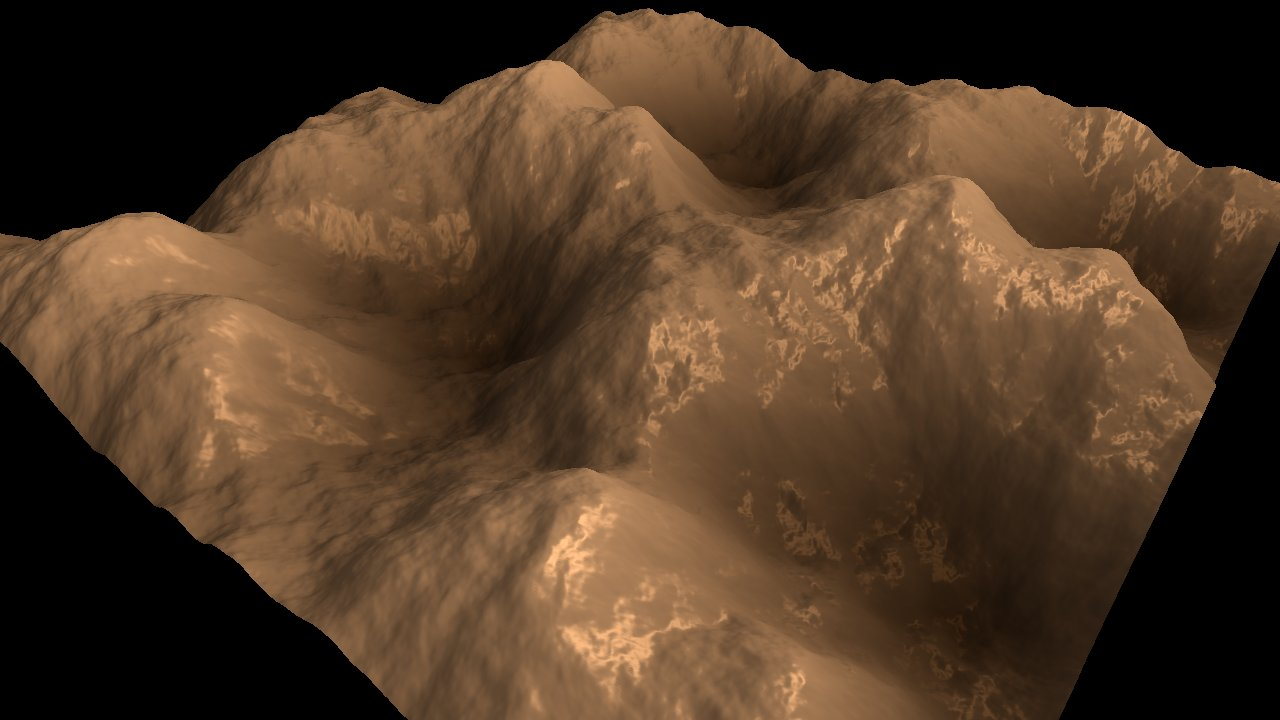
\includegraphics[width=0.49\textwidth]{images/fourier_24.jpg}}
	\subcaptionbox{Spektralsynthese mit Filter $f=1/f^{2.0}$\label{img.fourier20}} {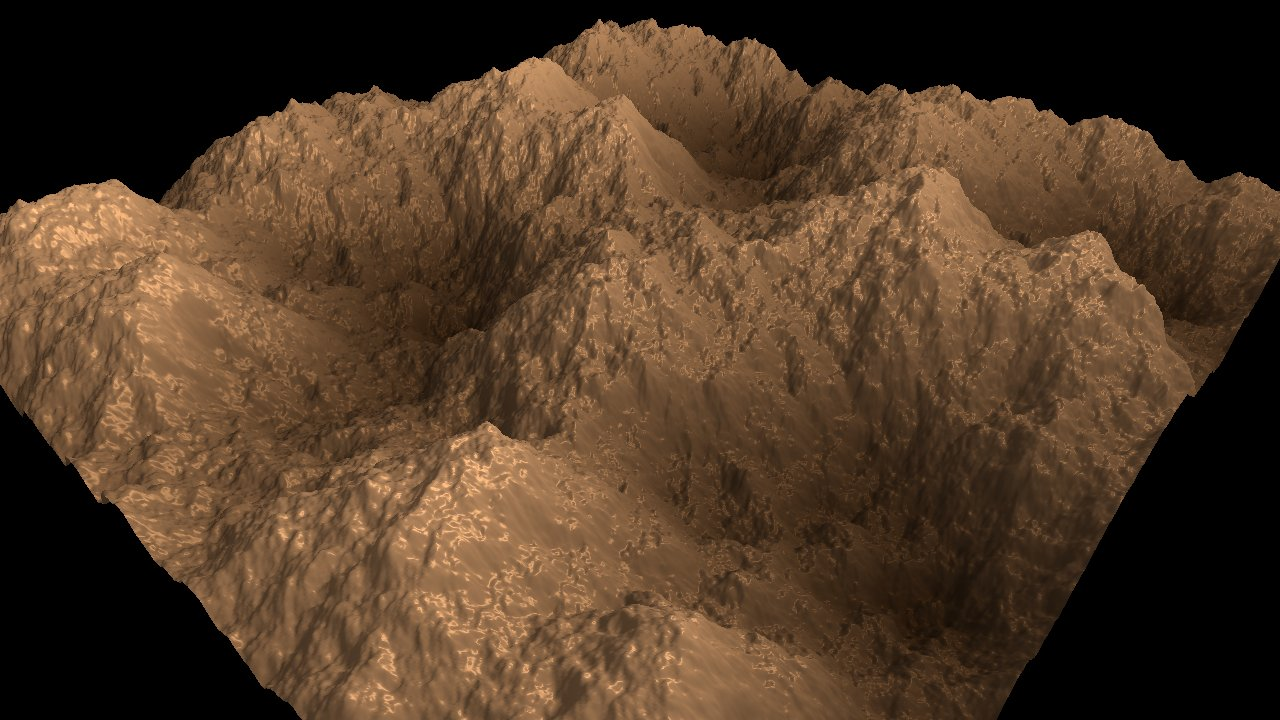
\includegraphics[width=0.49\textwidth]{images/fourier_20.jpg}}
	\caption{Durch Spektralsynthese erzeugte Höhenfelder in 3D gerendert. Bilder entnommen von: http://tinyurl.com/z6lfzmv}\label{img.fourierResult}
\end{figure}\label{test}

\subsection{Flexibilität}
Die Spektralsynthese ist sehr flexibel anpassbar, da sich mit der Änderung des Filters beliebig viele Effekte mit wenig Implementierungsaufwand erzeugen lassen. Klare Nachteile ergeben sich jedoch aus der genutzten Fourier bzw. der inversen Fourier Transformation, welche eine Auswertung innerhalb eines Frames nahezu unmöglich macht. Da die Frequenzen an jedem Ort des Höhenfeldes wirken hat das resultierende Gelände einen konstanten Detailgrad. Wünschenswert wäre es jedoch, die höherfrequenten Anteile in den tiefer liegenden Regionen nicht anzuzeigen, da Täler eher von lang geschwungenen Hügeln als von kantigen Felsformationen geprägt sind.\label{unisotrop}\footnote{Man spricht dann auch von heterogenem Terrain}. Im Vergleich zum Diamond-Square Algorithmus ist die Auflösung des Höhenfeldes jedoch irrelevant für die Funktionalität.

\subsection{Bewertung im Rahmen der Fragestellung}
Die Speicherung großer Geländeabschnitte erweist sich als einfach. Gespeichert werden muss nur das zugehörige Rauschbild\ref{fourier.rauschbild} sowie der verwendete Filter werden. Da das Rauschbild aus einem Pseudozufallsgenerator kommt, reicht hier auch der Seed aus womit sich der Speicheraufwand auf einige Bytes verringert.
Die Erzeugung einer nahezu unendlich großen Landschaft würde jedoch sehr viel Rechenzeit in Anspruch nehmen und müsste komplett im temporären Speicher gehalten werden. Eine Alternative wäre die Verwendung wie in \ref{Patches} vorgeschlagen, allerdings ist dies nicht möglich, da es keine Möglichkeit gibt einen glatten Übergang zwischen zwei Patches zu gestalten.